%%%%%%%%%%%%%%%%%%%% Paper.tex %%%%%%%%%%%%%%%%%%%%%%%%%%%%%%%%%%%
%
% ICCI 2026 submission, Springer conference template (svproc), as distributed by the conference.
% The preamble is the template's own; nothing has been added or removed.
%
%%%%%%%%%%%%%%%% Springer %%%%%%%%%%%%%%%%%%%%%%%%%%%%%%%%%%

\documentclass{svproc}
%\documentclass[graybox]{svmult}

% to typeset URLs, URIs, and DOIs
\usepackage{url}
\usepackage{helvet}         % selects Helvetica as sans-serif font
\usepackage{courier}        % selects Courier as typewriter font
%\usepackage{type1cm}        % activate if the above 3 fonts are
                           % not available on your system
\usepackage{color}
\usepackage{makeidx}         % allows index generation
\usepackage{graphicx}        % standard LaTeX graphics tool
\usepackage[misc]{ifsym}                            % when including figure files
\usepackage{multicol}        % used for the two-column index
\usepackage[bottom]{footmisc}% places footnotes at page bottom
\usepackage{tabularx}
\usepackage{multirow}
\usepackage{natbib}
\usepackage{algorithm}
\usepackage{algorithmic}
\usepackage[center]{caption}
\usepackage{longtable}
\usepackage{rotating}
 \usepackage{amsmath}
\usepackage{subfigure}
\usepackage[cp1251]{inputenc}
\def\UrlFont{\rmfamily}

\begin{document}
\renewcommand{\topfraction}{0.9}       % allow figures and tables to fill more of a page,
\renewcommand{\textfraction}{0.1}      % so that no large gaps are left below the text
\mainmatter              % start of a contribution
%
\title{Listening Through Ego-Noise: A Review of Acoustic Perception for Robots, Drones and Vehicles with Reproducible Case Studies}
%
\titlerunning{Acoustic Perception for Autonomous Systems}
%
% AUTHORS: replace before submission. Affiliation must contain only department, college/university, city, country.
% \author{First Author\inst{1} \and Second Author\inst{1}}
% %
% \authorrunning{First Author et al.}
% %
% \tocauthor{First Author, Second Author}
% %
% \institute{Department, University, City, Country\\
% \email{author@university.edu}}
\author{Heena Patel\and Kai Erik Hoff \and Linesh Raja \and
        Erlend Coates \and  Robin Bye}
%
\authorrunning{Heena et al.}
%
\tocauthor{Heena Patel, Kai Erik Hoff, Linesh Raja, Erlend Coates, Robin Bye}
%
\institute{Cyber-Physical Systems Laboratory, Department of ICT and Natural Sciences, NTNU - Norwegian University of Science and Technology, \AA{}lesund, Norway\\
\email{heena.s.patel@ntnu.no, kai.e.hoff@ntnu.no, linesh.raja@ntnu.no, erlend.coates@ntnu.no, robin.t.bye@ntnu.no}}
\maketitle              % typeset the title of the contribution

\begin{abstract}
Microphones allow robots, drones and road vehicles to detect events that cameras cannot see. However, the noise these machines generate themselves, known as ego-noise, often masks the sounds they need to hear. This paper reviews acoustic perception on such systems with a focus on ego-noise. It compares the acoustic conditions on robots, drones and vehicles. It then groups ego-noise suppression methods by the information about the noise they exploit. The main claims of the review are tested in reproducible case studies on three public datasets.
On a flying quadrotor, a learned spatial noise model raises the fraction of direction estimates within $10^\circ$ from 18\% to 60\%. Selecting the model by motor speed raises this further to 70\%. With this noise model, MVDR beamforming raises the SNR by 9.7\,dB over a single microphone, 5.7\,dB more than delay-and-sum.
Across five quadrotors, rotor tones carry between 1\% and 70\% of the noise energy. The highest values come from drones that were not flying. Yet a spatial noise model removes 6 to 13\,dB of noise on all of them.
In contrast, on a robot head in a quiet room, noise modeling lowers localization accuracy for moving speakers.
Based on these results, we propose four practical guidelines and identify open research problems.
\keywords{robot audition, drone audition, ego-noise, sound source localization, microphone arrays, embodied AI}
\end{abstract}

%=====================================================================================================
\section{Introduction}\label{sec:intro}
%=====================================================================================================
Sound gives autonomous systems a sense that works around corners, in the dark and in all directions.
A vehicle can hear an approaching car behind a blind corner more than a second before a camera-based detector sees it \cite{schulz2021hearing}.
A drone can search for people by their voices when they are hidden from its cameras \cite{deleforge2019spcup,gupta2025droneaudioset}.
An embodied agent finds a sounding object faster when it listens as well as looks \cite{chen2020soundspaces}.

Many of the required methods are already well established.
Classical array processing offers reliable tools for time delay estimation, subspace localization and beamforming \cite{knapp1976gcc,schmidt1986music,capon1969mvdr}.
Large pretrained models can recognize hundreds of sound classes \cite{gemmeke2017audioset,kong2020panns,gong2021ast}.
The main difficulty in deployment lies instead in the harsh acoustic conditions on board the machines themselves.
Robots, drones and vehicles move, vibrate and generate their own noise.
On a quadrotor, the rotor noise at the onboard microphones is often far louder than the target sound \cite{strauss2018dregon,ruizespitia2018aira}.

Research on robot audition began around 2000 with \emph{active audition}, the idea that a robot should move to hear better \cite{nakadai2000active}.
Several surveys have since reviewed sound source localization in robotics \cite{argentieri2015survey,rascon2017review}, deep learning-based localization \cite{grumiaux2022survey} and drone-based localization \cite{chevtchenko2025review}.
However, these surveys do not systematically compare ego-noise across robots, drones and vehicles.
They also do not link it to embodied audio-visual research in computer vision and machine learning.
Finally, none of them validates its conclusions experimentally.

To address these limitations, we review the literature with a focus on ego-noise and test the review's main claims in case studies on public data. The case studies answer three research questions.
\textbf{RQ1}: How much does explicit ego-noise modeling improve sound source localization, and what additional benefit does motor-state information provide?
\textbf{RQ2}: How consistent are ego-noise tonality and spatial structure across different drones?
\textbf{RQ3}: Under what conditions does explicit noise modeling fail to improve localization?

Our contributions are threefold.
First, we present an ego-noise-centered review of acoustic perception on autonomous systems (Sect.~\ref{sec:review}).
Second, we report reproducible evaluations on three public datasets (Sects.~\ref{sec:method} and \ref{sec:results}).
Third, we derive practical guidelines and research directions from both (Sect.~\ref{sec:discussion}).


%=====================================================================================================
\section{Literature Review}\label{sec:review}
%=====================================================================================================
\subsection{Acoustic conditions across robots, drones and vehicles}
\emph{Ground robots and humanoids} were the first systems studied in robot audition.
Early work addressed sound source localization and tracking while the robot moved its head, together with cancellation of its own motor noise \cite{nakadai2000active}.
Later mobile robots added real-time localization and tracking with onboard arrays \cite{valin2007tracking}.
On these robots, ego-noise comes mainly from the joint motors and changes with the joint state \cite{ince2009template}.

\emph{Aerial drones} are the most challenging case.
Their microphones are mounted tens of centimeters from rotors spinning at thousands of revolutions per minute.
The resulting noise combines harmonics of each rotor's shaft rate with broadband aerodynamic noise \cite{yen2023ncm}.
As a result, the signal-to-noise ratio (SNR) at the microphones is often far below 0\,dB \cite{ruizespitia2018aira,gupta2025droneaudioset}.
Search and rescue is the main application.
A recent systematic review found that 82\% of 49 drone audition studies targeted it, yet only three of the 49 ran in real time on board \cite{chevtchenko2025review}.

\emph{Road vehicles} use sound mainly for safety.
Applications range from detecting horns and sirens in urban traffic \cite{marchegiani2017urban} to detecting occluded vehicles from sound reflected by walls \cite{schulz2021hearing}.

\subsection{Sound source localization and tracking}
Generalized cross-correlation with phase transform (GCC-PHAT) estimates the time delay between each pair of microphones \cite{knapp1976gcc}.
Steered response power with phase transform (SRP-PHAT) sums these correlations over all pairs for every candidate direction \cite{dibiase2000srp}.
Subspace methods such as MUSIC separate the signal and noise subspaces of the spatial covariance matrix \cite{schmidt1986music}.
They usually assume that the noise is spatially white.
This assumption fails on robots and drones, where ego-noise is often correlated across microphones.
Generalized eigenvalue decomposition MUSIC (GEVD-MUSIC) removes the assumption by whitening the data with a noise covariance matrix.
On a robot, it kept localization reliable at 5 to 6\,dB lower SNR \cite{nakamura2011gevd}, and it later became the basis of early drone audition \cite{okutani2012quadrocopter,furukawa2013ncm}.

Learning-based localizers map multichannel features directly to source directions.
Deep networks combined with head movements resolve front-back ambiguity in binaural systems \cite{ma2017binaural}, and 3D convolutions over SRP maps track sources in reverberant rooms \cite{diazguerra2021cross3d}.
For tracking, particle filters link frame-wise estimates over time \cite{valin2007tracking}.
The LOCATA challenge benchmarks localization and tracking with both static and moving arrays \cite{evers2020locata}.
Table~\ref{tab:ssl} summarizes representative methods.

\begin{table}[t]
\centering
\scriptsize
\setlength{\tabcolsep}{4pt}
\caption{Representative localization methods and whether they model ego-noise or spatially structured noise.}
\label{tab:ssl}
\begin{tabular}{|l|c|l|l|c|}
\hline
\textbf{Method} & \textbf{Year} & \textbf{Key idea} & \textbf{Setting} & \textbf{Noise model} \\
\hline
GCC-PHAT \cite{knapp1976gcc} & 1976 & Pairwise time delay & Any array & No \\
MUSIC \cite{schmidt1986music} & 1986 & Signal and noise subspaces & Any array & No \\
SRP-PHAT \cite{dibiase2000srp} & 2000 & Steered response power & Any array & No \\
Valin et al. \cite{valin2007tracking} & 2007 & Beamformer, particle filter & Mobile robot & No \\
GEVD-MUSIC \cite{nakamura2011gevd} & 2011 & Noise-covariance whitening & Robot & Yes \\
Furukawa et al. \cite{furukawa2013ncm} & 2013 & Drone noise correlation matrix & Drone & Yes \\
Ma et al. \cite{ma2017binaural} & 2017 & Deep network, head movement & Binaural head  & No \\
Diaz-Guerra et al. \cite{diazguerra2021cross3d} & 2021 & 3D CNN on SRP maps & Static array & No \\
Wang and Cavallaro \cite{wang2022drone} & 2022 & Neural mask and SRP & Drone & Yes \\
Manamperi et al. \cite{manamperi2022drone} & 2022 & Delays, noise subtraction & Drone & Yes \\
\hline
\end{tabular}
\end{table}


\subsection{Event detection, separation and joint localization}
Large labeled collections such as AudioSet \cite{gemmeke2017audioset} enabled pretrained sound event detectors.
These range from convolutional networks \cite{kong2020panns} to the purely attention-based Audio Spectrogram Transformer \cite{gong2021ast}.
However, they are trained on web audio that rarely contains ego-noise.
This domain mismatch is a major obstacle when such models are deployed on robots, drones and vehicles.
For enhancement and separation, the minimum variance distortionless response (MVDR) beamformer \cite{capon1969mvdr} passes the target direction without distortion and minimizes the remaining noise power.
It requires an estimate of the noise covariance matrix, which links it directly to ego-noise modeling.
Sound event localization and detection (SELD) estimates the class, activity and direction of each event jointly \cite{adavanne2019seld}.
Its first public evaluation, in the Detection and Classification of Acoustic Scenes and Events (DCASE) challenge, showed that joint metrics can change the ranking of systems \cite{politis2021dcase}. Yet the DCASE SELD benchmarks use static arrays and contain no ego-noise.

\subsection{Ego-noise suppression}
Ego-noise differs from the interference assumed in most audio benchmarks.
It is loud and comes from fixed locations on the body.
It changes with every maneuver, yet it is partly predictable because the machine knows its own state.
Table~\ref{tab:egonoise} groups suppression methods by the information they exploit.
Spatial noise models learn the noise covariance from noise-only recordings and use it to whiten the data \cite{nakamura2011gevd,okutani2012quadrocopter}.
State-informed models also use the machine's own state.
Template subtraction selects a noise template according to the robot's joint status \cite{ince2009template}, motor data guide multichannel noise dictionaries \cite{schmidt2016dictionary,schmidt2018egonoise}, and on drones, flight sensor data predict the noise covariance \cite{furukawa2013ncm}.
On drones, rotor-noise-aware covariance estimation reports up to about 28\,dB of rotor-noise reduction \cite{yen2023ncm}.
Learned methods estimate masks that remove drone ego-noise before localization \cite{wang2022drone} or condition enhancement networks on rotor speed \cite{gulli2025rotor}.
Time-difference methods with noise subtraction also work at low SNR on irregular onboard arrays \cite{manamperi2022drone}.
Reference microphones placed near the propellers have already been used to guide multichannel enhancement \cite{tengan2022egonoise}.
Vibration sensors such as accelerometers near the motors could go further.
They record the phase of each rotor tone, which would allow tones to be cancelled rather than masked.
To our knowledge, such sensors have not yet been used for ego-noise suppression.

\begin{table}[t]
\renewcommand{\arraystretch}{1.05}
\centering
\scriptsize
\caption{Ego-noise suppression methods by the information they exploit.}
\label{tab:egonoise}
\begin{tabular}{|>{\raggedright\arraybackslash}p{3.8cm}|>{\raggedright\arraybackslash}p{5.5cm}|>{\raggedright\arraybackslash}p{2.4cm}|}
\hline
\textbf{Approach} & \textbf{Information used} & \textbf{Systems} \\
\hline
Spatial noise model \cite{nakamura2011gevd,okutani2012quadrocopter} & Noise-only recordings & Robots, drones \\
State-informed \cite{ince2009template,schmidt2016dictionary,schmidt2018egonoise,furukawa2013ncm,yen2023ncm} & Joint or motor state & Robots, drones \\
Learned \cite{wang2022drone,gulli2025rotor} & Paired training data, optionally rotor speed & Drones \\
Reference microphones \cite{tengan2022egonoise} & Noise recorded near the rotors & Drones \\
Vibration sensors (none yet) & Phase of each rotor tone & Open problem \\
\hline
\end{tabular}
\end{table}

\subsection{Audio in embodied and multimodal intelligence}
The vision and learning communities treat sound as one modality of an embodied agent.
SoundSpaces introduced navigation to sounding targets in scanned 3D environments \cite{chen2020soundspaces}, and its successor added continuous acoustic simulation \cite{chen2022soundspaces2}.
Move2Hear learns where an agent should move to separate a target sound from competing sounds \cite{majumder2021move2hear}.
For manipulation, fusing vision, audio and touch improves dense packing and pouring \cite{li2022seehearfeel}.
Audio-visual policies learned from in-the-wild human demonstrations with a contact microphone also generalize to unseen environments \cite{liu2024maniwav}.
Audio-language models now describe what is heard in open vocabulary \cite{tang2024salmonn}, and coupling a binaural spatial-audio encoder with a language model lets a system reason about where sounds come from \cite{zheng2024bat}.
However, these simulators and models usually omit the agent's own ego-noise.

Public data with real ego-noise are also limited.
DREGON provides in-flight drone recordings with per-rotor speeds and motion-capture ground truth \cite{strauss2018dregon}.
The IEEE Signal Processing Cup 2019 released drone recordings and ego-noise sets from ten teams \cite{deleforge2019spcup}, and AIRA-UAS records drone ego-noise during maneuvers \cite{ruizespitia2018aira}.
DroneAudioset adds 23.5 hours of recordings at SNRs from $-57.2$ to $-2.5$\,dB across drone types, throttle levels and microphone placements, although the drone is mounted on a fixed frame \cite{gupta2025droneaudioset}.
LOCATA provides static and moving arrays, including a robot head, with optical tracking \cite{lollmann2018locata,evers2020locata}.
To our knowledge, no public benchmark yet combines a moving machine, real ego-noise, its motor state, high-rate vibration sensing and realistic intermittent sources such as calls and whistles.

%=====================================================================================================
\section{Methodology}\label{sec:method}
%=====================================================================================================
\subsection{Review methodology}
The review covers acoustic perception on board moving, self-powered machines such as robots, drones and road vehicles.
It organizes the literature in three ways, by type of machine, by perception task and by the information each method exploits.
Methods developed for fixed arrays are included only where they transfer to moving machines.
The case studies then test the central claim of the review.
They use established methods, a single shared code base and three public datasets that differ in machine, array and noise conditions.

\subsection{Signal model and methods}
Consider an array of $M$ microphones at positions $\mathbf{r}_m$.
In the short-time Fourier transform (STFT) domain, at frequency $f$ and frame $t$, the array observes
\begin{equation}\label{eq:model}
\mathbf{x}(f,t)=\mathbf{a}(f,\mathbf{u})\,s(f,t)+\mathbf{n}(f,t),\qquad
a_m(f,\mathbf{u})=e^{\,j2\pi f\,\mathbf{r}_m^{\top}\mathbf{u}/c},
\end{equation}
where $s$ is the source signal arriving from unit direction $\mathbf{u}$, $\mathbf{n}$ contains ego-noise and environmental noise, and $c=343$\,m/s is the speed of sound.
The spatial covariance over the $T$ frames of a window is $\mathbf{R}_x(f)=\frac{1}{T}\sum_t\mathbf{x}(f,t)\mathbf{x}^{H}(f,t)$.

We compare five localizers that differ only in what they know about the noise.
(A) SRP-PHAT \cite{dibiase2000srp} sums the phase-transformed cross-spectra of all microphone pairs, steered to every candidate direction.
(B) SRP-PHAT with tone masking is a simple baseline of our own that builds on SRP-PHAT \cite{dibiase2000srp}.
It removes frequency bins at the blade passing harmonics $2kf_0$ of each rotor, where $f_0$ is the shaft rate from the motor log, since rotor noise contains strong tones at these frequencies \cite{yen2023ncm}.
A bin is removed when it rises at least 3\,dB above the local spectral floor, computed with a 4096-point STFT, and at most 40\% of the bins in the band are removed.
(C) MUSIC \cite{schmidt1986music} scores each direction using the noise subspace $\mathbf{E}_n(f)$ of $\mathbf{R}_x(f)$,
\begin{equation}\label{eq:music}
P(\mathbf{u})=\sum_{f}\frac{\tilde P_f(\mathbf{u})}{\max_{\mathbf{u}'}\tilde P_f(\mathbf{u}')},\qquad
\tilde P_f(\mathbf{u})=\big\|\mathbf{E}_n^{H}(f)\,\mathbf{a}(f,\mathbf{u})\big\|^{-2}.
% \qquad \hat{\mathbf{u}}=\arg\max_{\mathbf{u}}P(\mathbf{u}).
\end{equation}
Assuming a single source, $\mathbf{E}_n(f)$ holds the $M-1$ eigenvectors with the smallest eigenvalues.
Each narrowband pseudo-spectrum $\tilde P_f$ is normalized by its maximum over directions so that no single frequency bin dominates the sum, and the estimated direction is $\hat{\mathbf{u}}=\arg\max_{\mathbf{u}}P(\mathbf{u})$.
(D) GEVD-MUSIC \cite{nakamura2011gevd} takes $\mathbf{E}_n$ from the generalized eigenvectors of
\begin{equation}\label{eq:gevd}
\mathbf{R}_x(f)\,\mathbf{e}=\lambda\,\big(\mathbf{R}_n(f)+\delta\,\mathbf{I}\big)\,\mathbf{e}.
\end{equation}
This whitens the data with a noise covariance $\mathbf{R}_n$ learned from noise-only recordings.
The diagonal loading $\delta$ is set to $10^{-3}$ times the mean noise power.
(E) Speed-binned GEVD-MUSIC is a simple state-informed model, inspired by earlier work that adapts the noise model to the drone's state \cite{furukawa2013ncm,yen2023ncm}.
After discarding take-off and landing, it splits the noise-only frames into six quantile bins of mean rotor speed and learns one covariance per bin.
In each window, it uses the bin whose mean speed is closest to the mean rotor speed logged during that window.

For enhancement, we use the MVDR beamformer \cite{capon1969mvdr}
\begin{equation}\label{eq:mvdr}
\mathbf{w}(f)=\frac{\mathbf{R}_n^{-1}(f)\,\mathbf{a}(f,\hat{\mathbf{u}})}{\mathbf{a}^{H}(f,\hat{\mathbf{u}})\,\mathbf{R}_n^{-1}(f)\,\mathbf{a}(f,\hat{\mathbf{u}})}.
\end{equation}
It uses diagonal loading of $10^{-2}$ times the mean noise power and is steered towards the direction $\hat{\mathbf{u}}$ estimated by speed-binned GEVD-MUSIC (method E) rather than the ground-truth direction, which reflects realistic operation.


\subsection{Datasets, protocol and metrics}
\emph{DREGON} \cite{strauss2018dregon} provides recordings from an 8-microphone array (aperture 17\,cm) mounted on a quadrotor, sampled at 44.1\,kHz.
The measured speed of each rotor is logged at about 1\,kHz.
Noise models are learned from a 71\,s noise-only flight.
Evaluation uses two flights in which a loudspeaker plays white noise, one at high and one at low volume, giving 391 windows of 0.5\,s scored against motion capture.
The array and ground-truth frames are aligned once, using only SRP-PHAT (method A), on a separate recording made with the motors off (median residual $2.5^\circ$).
This alignment therefore cannot favor any of the compared methods.
For a controlled SNR experiment, 24 motors-off recordings (azimuth 45 to $90^\circ$, elevation 0 to $-30^\circ$) are each mixed with two different flight-noise segments at broadband SNRs from 0 to $-25$\,dB, giving 48 mixtures per level.
In this sweep, the noise model is learned on the first half of the noise-only flight, and the mixing noise is taken from the second half.
The unit of the motor log is undocumented.
Aligning the predicted rotor harmonics with the noise spectrum showed that it is revolutions per second.

\emph{SP Cup ego-noise} \cite{deleforge2019spcup} contains noise-only recordings contributed by ten teams, and we use four of the sets that provide 8-channel recordings of further quadrotors.
These are a DJI Phantom 4 Pro, an MK Quadro V3, an Intel Aero and a quadrotor recorded in an anechoic chamber.
Together with 50\,s of steady flight from the DREGON noise-only recording, this gives five drones in total.
For each drone, we measure two properties of the ego-noise that noise models rely on, its tonality and its spatial structure.
The \emph{tonal share} measures tonality.
It is the fraction of noise energy between 100 and 4000\,Hz that lies in spectral peaks at least 6\,dB above the noise floor, estimated with a running median over 300\,Hz.
It is computed on 1\,s segments and averaged.
We define the \emph{learned rejection} $G$ to measure spatial structure.
Following Wang and Cavallaro \cite{wang2016earinthesky}, we model quadrotor ego-noise as four directional sources (one per motor) plus a diffuse part.
Because the motors and microphones are fixed, these directions should stay stable.
We learn the four strongest noise eigenvectors on the first half of a recording.
These are then projected out of the second half, as in the eigencanceler \cite{haimovich1996eigencanceler}.
$G$ is the resulting drop in noise power in dB,
\begin{equation}\label{eq:rej}
G=-10\log_{10}\left(\frac{1}{F}\sum_{f}\frac{\mathrm{tr}\big(\mathbf{P}\,\mathbf{R}_2\,\mathbf{P}\big)}{\mathrm{tr}\,\mathbf{R}_2}\right),\qquad
\mathbf{P}=\mathbf{I}-\mathbf{U}_1\mathbf{U}_1^{H}.
\end{equation}
Here $\mathbf{U}_1(f)$ holds the four strongest eigenvectors of the noise covariance of the first half, $\mathbf{P}$ removes them, and $\mathbf{R}_2(f)$ is the covariance of the second half, over $F$ bins between 300 and 4000\,Hz.
A large $G$ means that the noise keeps arriving from a few stable directions, so a spatial model learned once remains valid.
For spatially white noise on eight microphones, $G=3$\,dB, since four of the eight dimensions hold half of the power.
Where the array geometry is published, we also compute $G$ for diffuse noise on the same array as a reference.

\emph{LOCATA} \cite{lollmann2018locata,evers2020locata} provides a 12-microphone robot-head array in a room with a reverberation time of about 0.5\,s.
The dataset is organized into six tasks, and we use the three that involve a single source.
These are a static loudspeaker with a static array (task 1), a moving talker with a static array (task 3) and a moving talker with a moving array (task 5).
Ground truth is computed in the array's own frame from optical tracking.
A window is scored when the source is active in at least 80\% of its samples, giving 396 windows.
For GEVD-MUSIC (method D), the noise covariance is learned from frames of the same recording in which the source is silent and at least 0.5\,s away from speech.
When fewer than 20 such frames exist, the 0.5\,s guard is dropped.

All localizers use the 300 to 4000\,Hz band and a $3^\circ$ grid of 7320 directions. They use a 1024-point STFT with 50\% overlap, except method B, which uses a 4096-point STFT with 75\% overlap throughout so that individual rotor tones are resolved; the subspace methods (C to E) use every second frequency bin.
Localization is scored by the angular error $e=\arccos(\mathbf{u}^{\top}\hat{\mathbf{u}})$, reported as the median and as the fraction of windows with $e\le10^\circ$.
Enhancement is scored by the SNR gain over a single microphone between 200 and 8000\,Hz.
The clean signal and the noise are beamformed separately, so the output SNR is computed exactly.
%=====================================================================================================
\section{Results}\label{sec:results}
%=====================================================================================================
\subsection{In-flight localization on a drone (RQ1)}
\begin{table}[t]
\renewcommand{\arraystretch}{1.05}
\centering
\scriptsize
\vspace{-15pt}
\caption{In-flight localization on DREGON (391 windows of 0.5\,s). Median and mean angular error, and fraction of windows within $10^\circ$ overall and per flight.}
\label{tab:dregon}
\begin{tabular}{|l|c|c|c|c|c|}
\hline
\textbf{Method} & \textbf{Median error} & \textbf{Mean error} & \textbf{Within $10^\circ$} & \textbf{Loud source} & \textbf{Quiet source} \\
\hline
A SRP-PHAT & $76.7^\circ$ & $72.7^\circ$ & 18.4\% & 36.1\% & 1.5\% \\
B SRP-PHAT + tone mask & $67.3^\circ$ & $59.5^\circ$ & 33.0\% & 58.6\% & 8.5\% \\
C MUSIC & $72.4^\circ$ & $67.4^\circ$ & 23.3\% & 44.5\% & 3.0\% \\
D GEVD-MUSIC, one model & $6.1^\circ$ & $31.4^\circ$ & 60.4\% & 74.9\% & 46.5\% \\
E GEVD-MUSIC, speed-binned & $\mathbf{5.0^\circ}$ & $\mathbf{22.7^\circ}$ & \textbf{69.8\%} & \textbf{75.9\%} & \textbf{64.0\%} \\
\hline
\end{tabular}
\end{table}
Table~\ref{tab:dregon} shows that without a noise model, SRP-PHAT (A) and MUSIC (C) have median errors above $70^\circ$.
Their response peaks on rotor noise arriving from above the array, at about 45 to $50^\circ$ elevation (Fig.~\ref{fig:tracking}).
Learning the noise covariance 
(D) reduces the median error from $76.7^\circ$ to $6.1^\circ$.
Selecting the covariance by motor speed (E) raises the fraction within $10^\circ$ by a further 9.4 percentage points and reduces the mean error from $31.4^\circ$ to $22.7^\circ$.
This gain is concentrated on the quiet-source flight, where E reaches 64.0\% within $10^\circ$ against 46.5\% for D.
Masking rotor tones (B) raises the fraction of SRP-PHAT within $10^\circ$ from 18.4\% to 33.0\%, but two thirds of the windows still exceed $10^\circ$ of error.
The reason is that much of the noise lies between the tones.
In the 1 to 2\,kHz band, the predicted blade passing tones cover 34\% of the frequency bins but hold only 42\% of the noise energy.
% \vspace{-50pt}
\begin{figure}[t]
\centering
% \vspace{-pt}
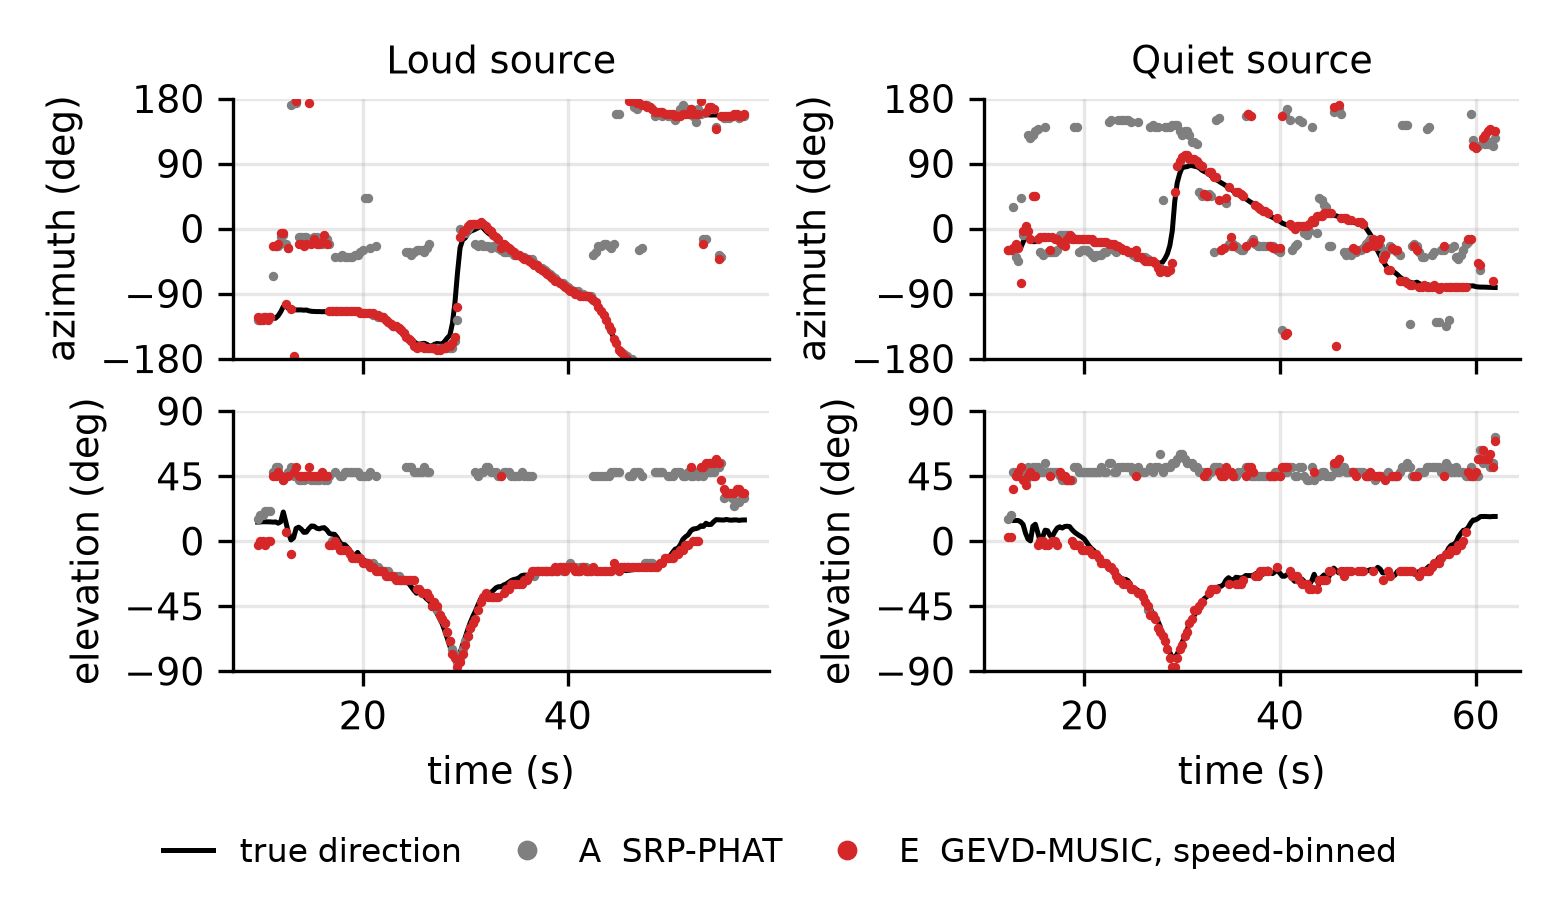
\includegraphics[width=0.66\textwidth]{fig/dregon_tracking.png}
\caption{True source direction (black) against SRP-PHAT (gray) and speed-binned GEVD-MUSIC (red) over the two DREGON flights. SRP-PHAT locks onto rotor noise at about 45 to $50^\circ$ elevation.}
\label{fig:tracking}
\end{figure}
\begin{table}[b]
\renewcommand{\arraystretch}{1.05}
\centering
\scriptsize
\vspace{-10pt}
\caption{Fraction of trials within $10^\circ$ for motors-off recordings mixed with held-out flight noise (48 mixtures per level).}
\label{tab:snr}
\begin{tabular}{|l|c|c|c|c|c|c|}
\hline
\textbf{Method} & \textbf{0\,dB} & \textbf{$-5$\,dB} & \textbf{$-10$\,dB} & \textbf{$-15$\,dB} & \textbf{$-20$\,dB} & \textbf{$-25$\,dB} \\
\hline
A SRP-PHAT & 100\% & 98\% & 40\% & 2\% & 0\% & 0\% \\
B SRP-PHAT + tone mask & 100\% & 100\% & 46\% & 2\% & 0\% & 0\% \\
C MUSIC & 100\% & 98\% & 46\% & 0\% & 0\% & 0\% \\
D GEVD-MUSIC, one model & 100\% & 100\% & \textbf{90\%} & 29\% & 0\% & 0\% \\
E GEVD-MUSIC, speed-binned & 100\% & 100\% & \textbf{90\%} & \textbf{35\%} & 0\% & 0\% \\
\hline
\end{tabular}
\end{table}

% \vspace{-10pt}
Table~\ref{tab:snr} shows how the methods degrade as the drone noise becomes louder.
At $-10$\,dB, the noise-model methods (D, E) still localize 90\% of trials within $10^\circ$, while the others fall to 40 to 46\%.
At $-15$\,dB, they keep 29 to 35\% against at most 2\% for the others.
From $-20$\,dB, every method fails.
The noise model therefore delays the collapse of accuracy by about 5\,dB.
The learned noise covariance also improves the recovered signal.
Over 48 mixtures at $-10$\,dB, beamforming towards the direction estimated by E raises the SNR over a single microphone by a median of 4.0\,dB with delay-and-sum.
MVDR raises it by 9.1\,dB with one noise covariance and by 9.7\,dB with the speed-binned covariance, with the largest gains between 1 and 4\,kHz (Fig.~\ref{fig:snrfreq}).
\begin{figure}
\vspace{-20pt}
\centering
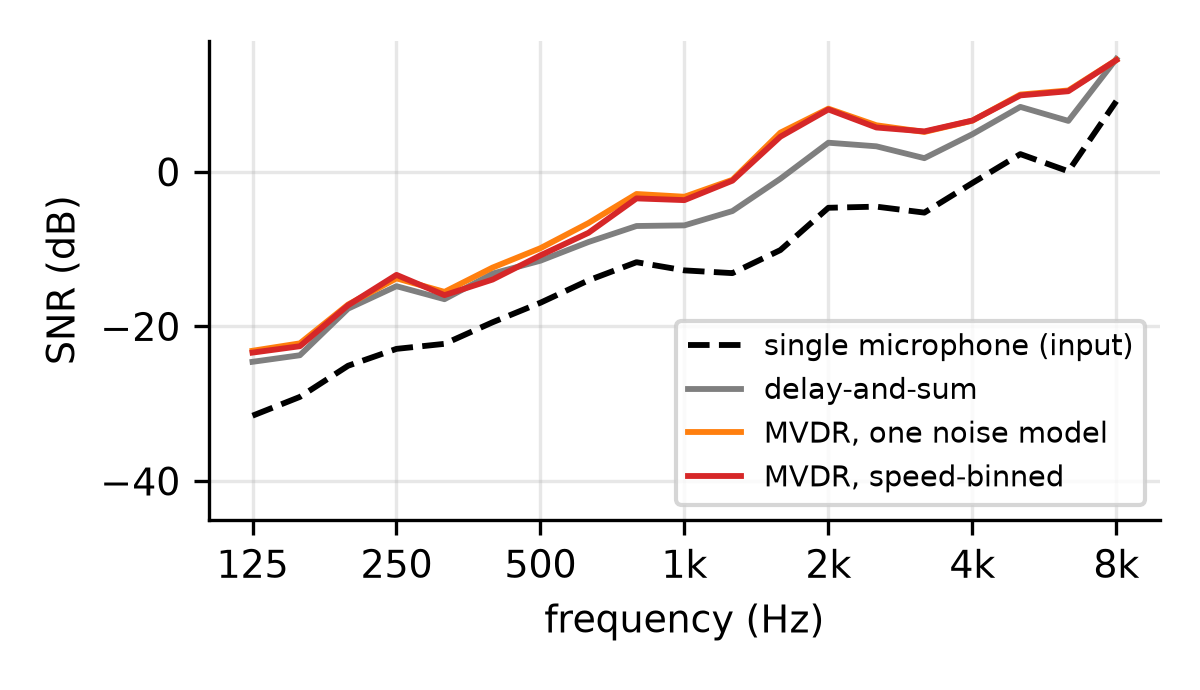
\includegraphics[width=0.58\textwidth]{fig/dregon_snr_by_frequency.png}
\vspace{-10pt}
\caption{SNR in third-octave bands for a single microphone (dashed) and after beamforming towards the direction estimated by method E, pooled over 48 mixtures at $-10$\,dB broadband input SNR.}
\label{fig:snrfreq}
\end{figure}
\vspace{-30pt}
\subsection{Ego-noise across five drones (RQ2)}
% Fig.~\ref{fig:drones} shows that the tonal share differs by a factor of about 60 between drones, although the difference is reduced to about 15 when discounting drones which were not in self-powered flight.
% It ranges from 1.2\% of the noise energy on the Intel Aero, through 15.7\% on DREGON, to 69.7\% on the MK Quadro V3.
% However, the two highest values come from drones that were not in self-powered flight.  Among the three flying drones, the tonal share differs by a factor of about 13.
% In flight, the controller continually adjusts the rotor speeds. This smears the rotor harmonics.
% We measured the rotor-speed variation in each 1\,s window of the DREGON flight as the standard deviation of the logged speeds. Windows with more variation have a lower tonal share (Spearman $\rho=-0.34$, $p=0.016$, 50 windows). At the same mean rotor speed, their harmonic peaks are also lower (Fig.~\ref{fig:jitter}). Tone-based methods are therefore valuable on some drones and nearly irrelevant on others. Moreover, tonality measured on a drone that is not flying can overstate the tonality in flight.
Fig.~\ref{fig:drones} shows that the tonal share differs by a factor of about 60 between drones. It ranges from 1.2\% of the noise energy on the Intel Aero, through 15.7\% on DREGON, to 69.7\% on the MK Quadro V3.
However, the two highest values come from drones that were not in self-powered flight.
They are marked with an asterisk (*) in Fig.~\ref{fig:drones}.
Among the three flying drones, the tonal share differs by a factor of about 13.
Tone-based methods are therefore valuable on some drones and nearly irrelevant on others.
In flight, the controller continually adjusts the rotor speeds.
This smears the rotor harmonics.
We measured the rotor-speed variation in each 1\,s window of the DREGON flight as the standard deviation of the logged speeds.
Windows with more variation have a lower tonal share (Spearman $\rho=-0.34$, $p=0.016$, 50 windows).
At the same mean rotor speed, their harmonic peaks are also lower (Fig.~\ref{fig:jitter}).
Tonality measured on a drone that is not flying can therefore overstate the tonality in flight.

In contrast, the learned rejection $G$ (Eq.~\ref{eq:rej}) is 6.0 to 12.9\,dB on every drone, well above the 3\,dB expected for white noise.
On the DREGON and MK Quadro arrays, with apertures of 17 and 15\,cm, the rejection exceeds that of diffuse noise on the same array by 4.5 and 2.7\,dB.
Rotor noise is thus spatially more structured than ordinary background noise.
On the 6\,cm DJI Phantom array, a spatial model removes less ego-noise than diffuse noise (8.2 against 19.0\,dB).
This suggests that the noise is uncorrelated between the microphones. Airflow over each microphone capsule may cause this.
\begin{figure}[H]
\centering
\vspace{-15pt}
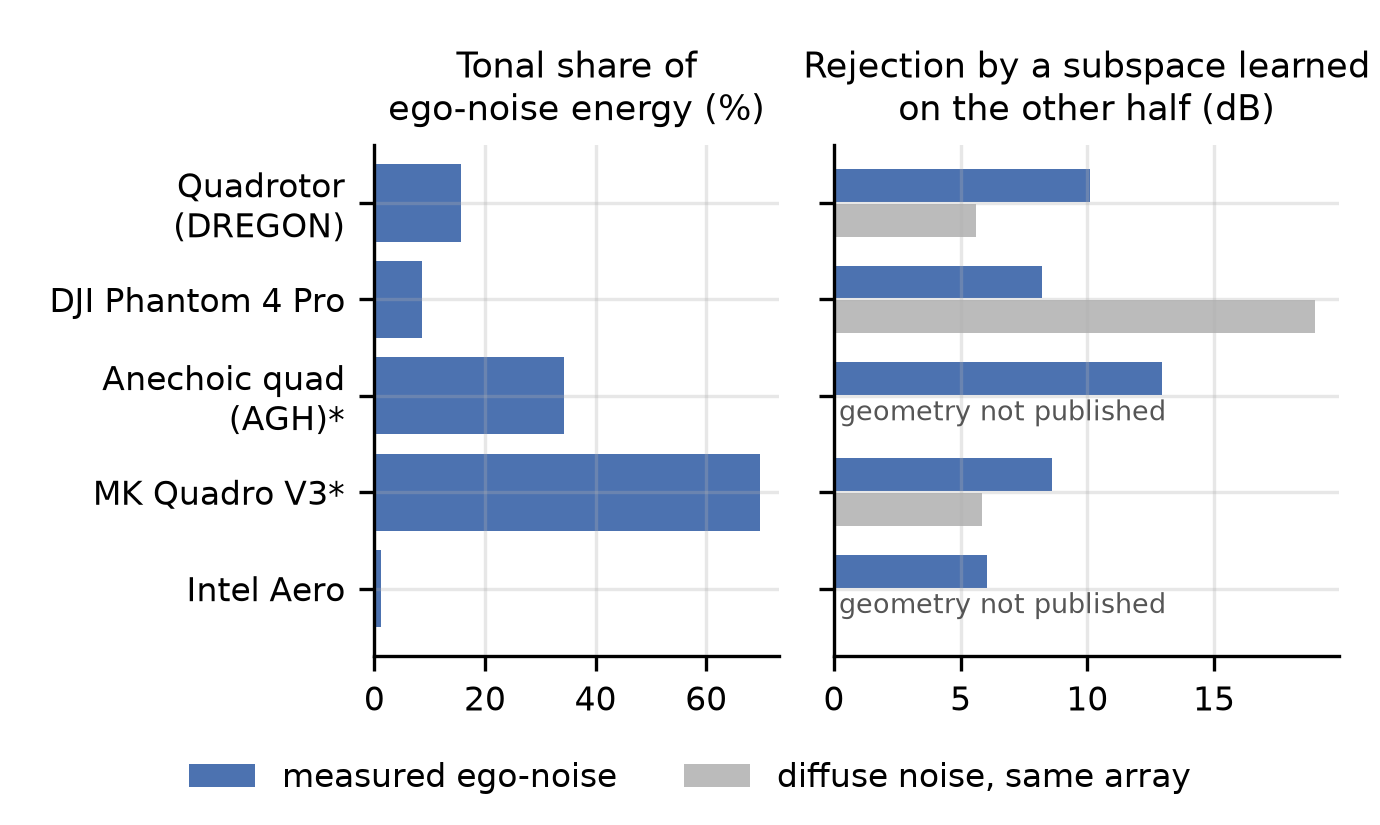
\includegraphics[width=0.58\textwidth]{fig/multidrone_egonoise.png}
\caption{Ego-noise of five quadrotors. Left, tonal share of the noise energy. Right, noise removed by a spatial subspace learned on the other half of the recording, with diffuse noise on the same array as a reference. 
* represents a drone that was not flying during the recording. The MK Quadro V3 was held about 0.5\,m above the floor. The AGH quadrotor stood still in an anechoic chamber.}
\label{fig:drones}
\end{figure}
\begin{figure}[H]
\centering
\vspace{-25pt}
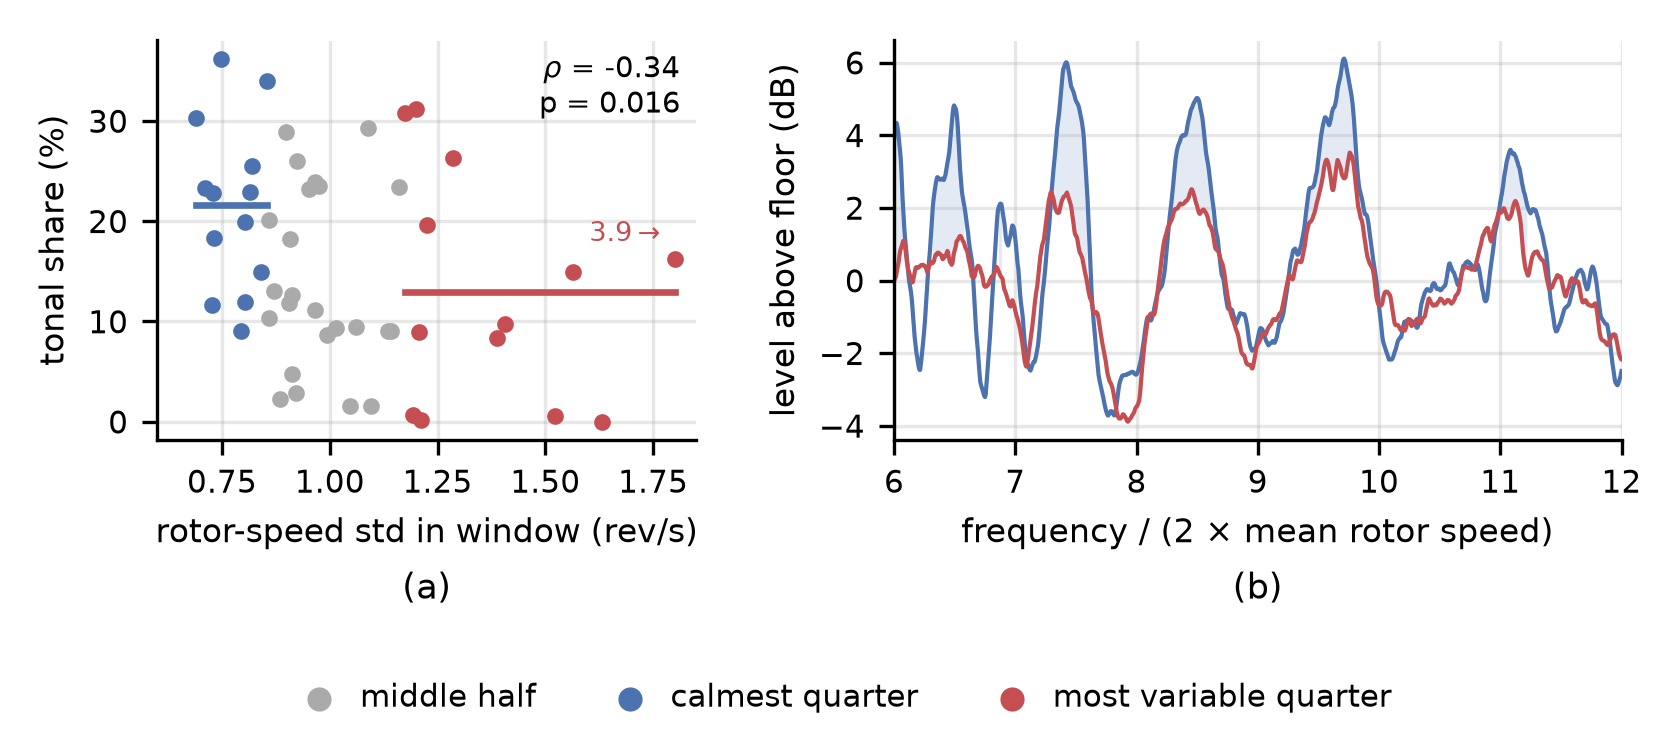
\includegraphics[width=0.9\textwidth]{fig/dregon_jitter_tonal.png}
\caption{Rotor-speed variation and tonal share in the DREGON noise-only flight (50 windows of 1\,s). (a) Tonal share against the standard deviation of the rotor speeds within each window, averaged over the four rotors. Horizontal lines mark the means of the calmest and the most variable quarter of the windows (21.6\% and 12.9\%); one window with 3.9\,rev/s is drawn at the edge. (b) Mean spectrum of these two quarters, with each window aligned to its own mean rotor speed. Both quarters have the same mean speed (80.7 and 80.8\,rev/s), but the harmonic peaks are lower in the variable windows (shaded).}
\label{fig:jitter}
\end{figure}

\subsection{A robot-head array without ego-noise (RQ3)}
Table~\ref{tab:locata} shows that the classical localizers are accurate on the robot-head array, even when both the talker and the array move.
With a static loudspeaker (task 1), all methods localize every window within $10^\circ$.
With moving talkers, however, the noise model does not help.
It lowers the fraction within $10^\circ$ by 18 to 33 percentage points relative to SRP-PHAT, with or without the 0.5\,s guard.
The SNR at the array is 16 to 25\,dB, and the background noise is close to diffuse.
Its four strongest spatial components hold 75 to 89\% of its energy, against 79\% for a diffuse field on the same array.
Whitening with the covariance of such weak, unstructured noise therefore distorts the spatial spectrum more than it suppresses noise.
\begin{table}[]
\renewcommand{\arraystretch}{1.05}
\centering
\scriptsize
\vspace{-25pt}
\caption{LOCATA robot-head array. Fraction of windows within $10^\circ$ and median error, with window counts in parentheses.}
\label{tab:locata}
\begin{tabular}{|l|c|c|c|}
\hline
\textbf{Method} & \textbf{Task 1 (34)} & \textbf{Task 3 (151)} & \textbf{Task 5 (211)} \\
\hline
A SRP-PHAT & 100\% / $4.8^\circ$ & \textbf{91.4\%} / $2.8^\circ$ & \textbf{99.1\%} / $2.8^\circ$ \\
C MUSIC & 100\% / $3.1^\circ$ & 86.1\% / $3.2^\circ$ & 95.7\% / $2.8^\circ$ \\
D GEVD-MUSIC, 0.5\,s guard & 100\% / $3.2^\circ$ & 69.5\% / $5.4^\circ$ & 68.2\% / $4.0^\circ$ \\
D GEVD-MUSIC, no guard & 100\% / $2.8^\circ$ & 58.3\% / $8.0^\circ$ & 81.0\% / $4.6^\circ$ \\
\hline
\end{tabular}
\end{table}
\vspace{-20pt}
%=====================================================================================================
\section{Discussion}\label{sec:discussion}
%=====================================================================================================
\emph{Answers to the research questions.}
\textbf{RQ1.} When ego-noise dominates and is spatially structured, an explicit noise model gives the largest improvement of all compared methods, for both localization and enhancement.
The motor state adds most when the target is weak, which is the typical case in search and rescue.
This agrees with earlier robot and drone studies \cite{nakamura2011gevd,furukawa2013ncm,yen2023ncm}.
\textbf{RQ2.} Ego-noise is only partly consistent across drones.
A fixed spatial model removes ego-noise on all five drones, but tonality varies widely between them.
On the small 6\,cm array, where airflow noise appears to dominate, the model removes less noise than it would from a diffuse field.
\textbf{RQ3.} A noise model can also hurt.
On the robot head, at high SNR and with nearly diffuse noise, it lowered accuracy for moving talkers.

\emph{Practical guidelines.}
(1) Record a short noise-only segment and learn a spatial noise model. In our controlled SNR experiment, about 35\,s of flight was sufficient.
(2) Measure the tonal share of the noise before investing in tone masking.
(3) Prefer larger arrays and shield the microphones from airflow. In our data, only the arrays of 15\,cm or more showed ego-noise more structured than diffuse noise.
(4) Check the SNR and how diffuse the background is before applying a noise model, and always report a baseline without it.

\emph{Research directions.}
Drone recordings can reach SNRs as low as $-57$\,dB \cite{gupta2025droneaudioset}, far below the $-20$\,dB at which every method compared here fails.
Such conditions call for noise models that follow each rotor's speed continuously \cite{yen2023ncm}, combined with learned suppression \cite{wang2022drone,gulli2025rotor}.
In DREGON, the flight controller's inertial sensor is logged at about 1\,kHz and therefore cannot observe vibration above about 500\,Hz, whereas localization uses 300 to 4000\,Hz.
A dedicated high-rate vibration sensor near each motor could supply the phase of the rotor tones, so that they are subtracted rather than masked.
A spatial model learned on one half of a recording remained valid on the other half for every drone, which suggests that short calibration flights may suffice for new drones.
Finally, embodied simulators \cite{chen2022soundspaces2} should model ego-noise that depends on motor state, and new benchmarks should include real ego-noise together with motor state.

\emph{Threats to validity.}
Our study has four main limitations.
First, the target sources in the drone experiments are loudspeakers playing white noise, which is easier to localize than speech or calls.
Second, only DREGON provides rotor speeds, so the benefit of state information is shown on a single drone.
Third, the robot-head results come from one array in one room, so RQ3 should be confirmed in other settings.
Fourth, with 48 trials per SNR level, differences of a few percentage points in the controlled SNR experiment are within noise.

%=====================================================================================================
\section{Conclusion}\label{sec:con}
%=====================================================================================================
This paper reviewed acoustic perception for robots, drones and road vehicles and identified ego-noise as the central obstacle to reliable hearing on these machines.
Case studies on three public datasets supported this view.
On a flying drone, a learned noise model raised the fraction of direction estimates within $10^\circ$ from 18\% to 60\%, and selecting it by motor speed raised this to 70\%.
With the same noise model, MVDR beamforming more than doubled the SNR gain of delay-and-sum (9.7 against 4.0\,dB).
Across five quadrotors, a spatial noise model removed 6 to 13\,dB of noise, although their tonal share varied from 1\% to 70\%.
In contrast, on a robot-head array in a quiet room, where ego-noise is absent, noise modeling lowered accuracy for moving talkers.
Future work should combine motor speed with high-rate vibration sensing and evaluate realistic sources such as speech, calls and whistles.
%
% Bibliography
%
\renewcommand{\bibsection}{\section*{References}} % references continue on the same page
\renewcommand{\bibfont}{\small}                    % Springer reference size (9 pt)
\setlength{\bibsep}{0pt}                          % no extra space between references
\bibliographystyle{plain}
\bibliography{ref}

\end{document}
